\documentclass{article}
\usepackage[a4paper, margin = 1.9cm]{geometry}
\usepackage[english]{babel}
\usepackage{float}
\usepackage{graphicx}
\usepackage{gensymb}
\usepackage{csquotes}

\title{Pseudo code for mobile robot}
\author{Lennart Großkreutz}
\date{\today}

\usepackage{algorithm2e}

\begin{document}

\maketitle

\section{Definitions}
We use the term \textit{center line} to describe the line depicted in the graphic below: \\
\hspace{10mm}

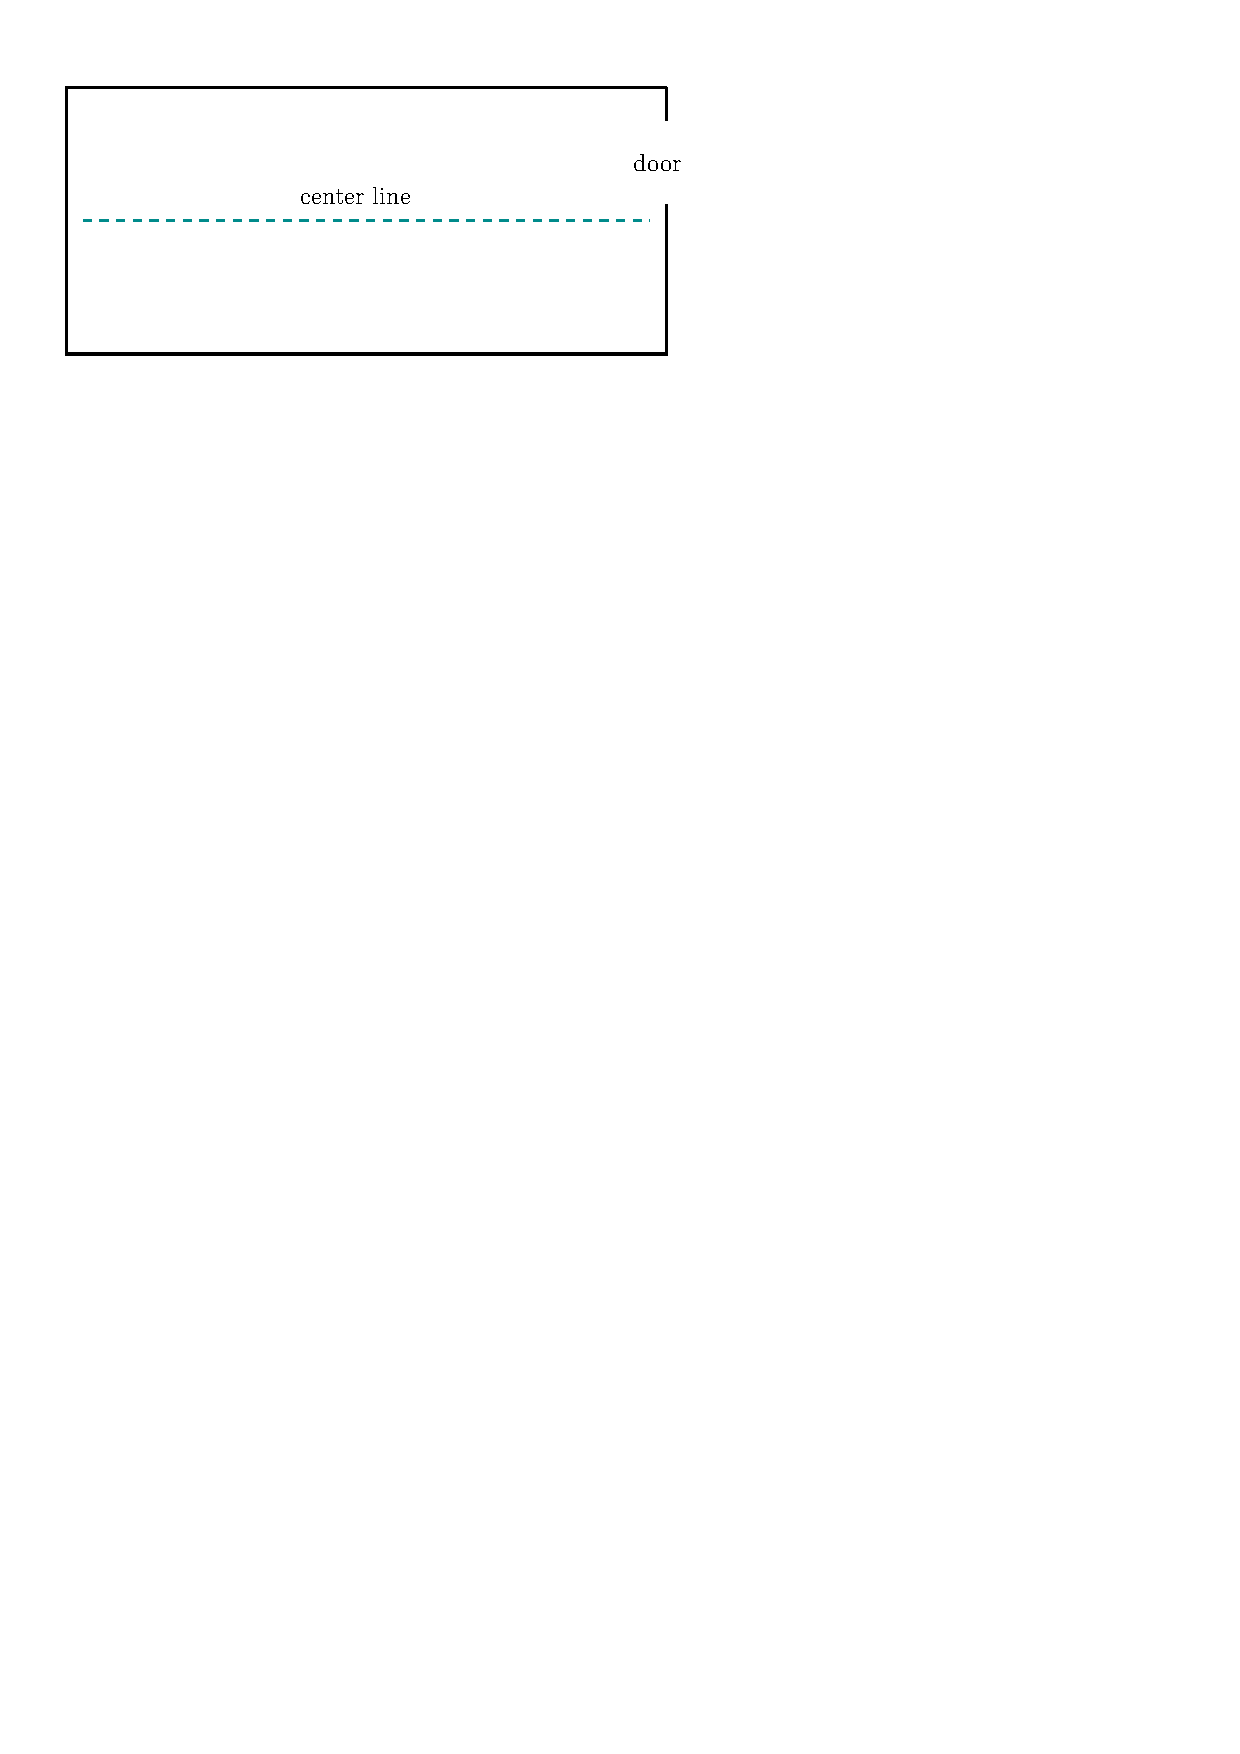
\includegraphics[width=.6\textwidth]{images/center-line.pdf}

\section{Algorithm}

\begin{algorithm}[H]
	%\DontPrintSemicolon
	\KwData{none}
	\KwResult{robot leaves the room through the open door without touching any obstacles}
	\BlankLine
	\While{door not yet passed}{
		measurements $\longleftarrow$ scan()\;
		gradually make a full rotation by storing the current sensor data and then rotating around a fixed angle $\phi$\;
		\uIf{door-like pattern detected in measurements}{
			rotate so that the robot is looking in the supposed direction of the door\;
			move forward a fixed distance $d_{door}$\;
		}
		\uElseIf{robot assumed to be on center line after analysing measurements}{
			assure robot is alligned with center line\;
			\uIf(\tcp*[f]{wall reached with no door: door on the other side}){wall ahead}{turn 180 \degree}
			\uElse{follow center line for some fixed distance $d_{center line}$}
		}
		\uElseIf{two parallel walls detected in measurements}{
			rotate so that center line is in sight with no obstacles in between\;
			move a fixed distance $d_{searching}$ towards center line
		}
		\uElse(\tcp*[f]{no clue where robot is in the room}){
			\While{nearby obstacle in gaze direction}
				{rotate by a random angle in a fixed range $[ \alpha, \beta]$}
		}
		move forward a fixed distance $d_{random}$
	}
	\caption{Room escape}
\end{algorithm}

\section{Sub-Routine \textit{scan()}}
The robot gradually does a full rotation, meanwhile creating a list of measurements. 
It stores the current distance captured by the sensor, then it rotates for a fixed angle
$\phi$ (e.g. $\phi = 1 \degree$) until the robot has completed a full rotation.
$\phi$ should be chosen as divider of $2 \pi = 360 \degree$ so that the robot returns to the original gaze direction after the scan.

\section{Technical remarks}
\begin{itemize}
	\item The robot does never know certainly whether it passed the door, so the outer loop is rather \enquote{while(true)}. The robot is stopped externally as soon as it passed the door. 
	\item TODO what is a door-like pattern
\end{itemize}


\end{document}